\documentclass[border=4pt]{standalone}

\usepackage{amsmath}
\usepackage{tikz}
\usepackage{mathdots}
\usepackage{yhmath}
\usepackage{cancel}
\usepackage{color}
\usepackage{siunitx}
\usepackage{array}
\usepackage{multirow}
\usepackage{amssymb}
\usepackage{gensymb}
\usepackage{tabularx}
\usepackage{booktabs}
\usetikzlibrary{fadings}
\usetikzlibrary{patterns}


\begin{document}
 



\tikzset{every picture/.style={line width=0.75pt}} %set default line width to 0.75pt        

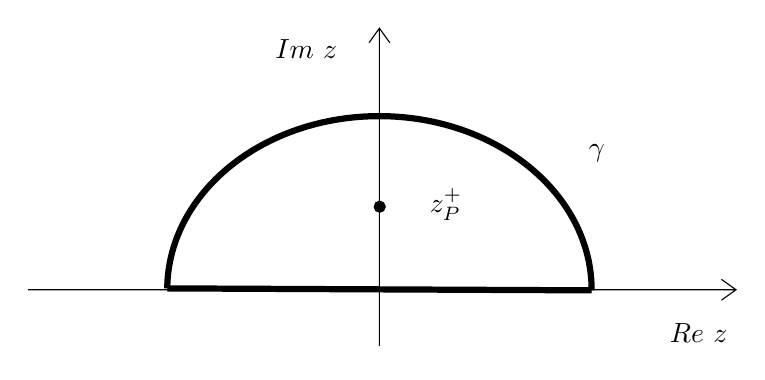
\begin{tikzpicture}[x=0.75pt,y=0.75pt,yscale=-1,xscale=1]
%uncomment if require: \path (0,300); %set diagram left start at 0, and has height of 300

%Shape: Axis 2D [id:dp8732382545113653] 
\draw  (50,181) -- (391,181)(219.21,55) -- (219.21,208) (384,176) -- (391,181) -- (384,186) (214.21,62) -- (219.21,55) -- (224.21,62)  ;
%Shape: Arc [id:dp2660318379597453] 
\draw  [draw opacity=0][line width=2.25]  (116.98,180.34) .. controls (117.37,134.33) and (163.12,97.21) .. (219.41,97.35) .. controls (275.87,97.49) and (321.55,135.05) .. (321.44,181.25) .. controls (321.44,181.26) and (321.44,181.27) .. (321.44,181.29) -- (219.21,181) -- cycle ; \draw  [line width=2.25]  (116.98,180.34) .. controls (117.37,134.33) and (163.12,97.21) .. (219.41,97.35) .. controls (275.87,97.49) and (321.55,135.05) .. (321.44,181.25) .. controls (321.44,181.26) and (321.44,181.27) .. (321.44,181.29) ;
%Shape: Circle [id:dp6436565637870435] 
\draw  [fill={rgb, 255:red, 0; green, 0; blue, 0 }  ,fill opacity=1 ] (216.67,141) .. controls (216.67,139.53) and (217.86,138.33) .. (219.33,138.33) .. controls (220.81,138.33) and (222,139.53) .. (222,141) .. controls (222,142.47) and (220.81,143.67) .. (219.33,143.67) .. controls (217.86,143.67) and (216.67,142.47) .. (216.67,141) -- cycle ;
%Straight Lines [id:da134917536451582] 
\draw [line width=2.25]    (116.98,180.34) -- (321.44,181.29) ;



% Text Node
\draw (184,65) node    {$Im\ z$};
% Text Node
\draw (373,202) node    {$Re\ z$};
% Text Node
\draw (324,115) node    {$\gamma $};
% Text Node
\draw (251.33,140) node    {$z^{+}_{P}$};


\end{tikzpicture}

\end{document}
